\documentclass[10pt]{article}

% Lines beginning with the percent sign are comments
% This file has been commented to help you understand more about LaTeX

% DO NOT EDIT THE LINES BETWEEN THE TWO LONG HORIZONTAL LINES

%---------------------------------------------------------------------------------------------------------

% Packages add extra functionality.
\usepackage{times,graphicx,epstopdf,fancyhdr,amsfonts,amsthm,amsmath,algorithm,algorithmic,xspace,hyperref}
\usepackage[left=1in,top=1in,right=1in,bottom=1in]{geometry}
\usepackage{sect sty}	%For centering section headings
\usepackage{enumerate}	%Allows more labeling options for enumerate environments 
\usepackage{epsfig}
\usepackage[space]{grffile}
\usepackage{booktabs}
\usepackage{forest}
\usepackage{enumitem}   
\usepackage{fancyvrb}
\usepackage{todonotes}
\usepackage{array}

% This will set LaTeX to look for figures in the same directory as the .tex file
\graphicspath{.} % The dot means current directory.

\pagestyle{fancy}

\lhead{Final Project}
\rhead{\today}
\lfoot{CSCI 334: Principles of Programming Languages}
\cfoot{\thepage}
\rfoot{Spring 2024}

% Some commands for changing header and footer format
\renewcommand{\headrulewidth}{0.4pt}
\renewcommand{\headwidth}{\textwidth}
\renewcommand{\footrulewidth}{0.4pt}

% These let you use common environments
\newtheorem{claim}{Claim}
\newtheorem{definition}{Definition}
\newtheorem{theorem}{Theorem}
\newtheorem{lemma}{Lemma}
\newtheorem{observation}{Observation}
\newtheorem{question}{Question}

\setlength{\parindent}{0cm}

%---------------------------------------------------------------------------------------------------------

% DON'T CHANGE ANYTHING ABOVE HERE

% Edit below as instructed

\title{frisBetterRunningOffense (frisBRO) Language Specification} % Replace SnappyLanguageName with your project's name

\author{Skylar Yarter \and Jocelyn Bliven} % Replace these with real partner names.

\begin{document}
  
\maketitle

\subsection*{Introduction}

In the middle of an ultimate frisbee game, there are countless split-second decisions to make based on a wide variety of factors. It can be stressful and confusing for coaches and players alike. No longer! frisBRO helps a user decide what ultimate frisbee play to call in a given situation based on where the players, disc, and the defensive force are. 
~\\
~\\
Ultimate frisbee requires “reading” the field to figure out what play is best to call. This reading of the field requires evaluating multiple parameters. A language that allows the user to read the field more easily and without human emotion and bias swaying the result would allow more appropriate plays to be called. Many of the evaluations being made by the players or coaches when choosing a play are quantitative (e.g. where are the players and disc on the field, which way is the defense forcing). These quantitative parameters fit well within the scope of a programming language and can be compared better by a computer than a person standing on the field with a skewed perspective.


\subsection*{Design Principles}

We aim to create an easily readable, quick-to-type programming language so it can be used by frisbee coaches and players, who may not be familiar with general programming practices. Therefore, we prioritize simplicity in the syntax of our language so that it is easy to learn and to read. We do not want to overcomplicate the language by adding too many elements or rules, as that would hinder our user base. The language need not be object-oriented or follow a complex model as it is fairly basic, which allows for the easy-to-learn syntax. We also wanted to make the language quickly usable as this is designed to be used in the middle of a frisbee game.  

\subsection*{Examples}
    The program takes in a txt file and returns an svg file.
    
    ~\\
    ~\\
    Example 1: Basic use (basic.txt)
    ~\\
    \begin{verbatim}
    Offense = {(120,390), true; (140,220), false; (160,220), false; (180,220), false; 
                (200,220), false; (220,220), false; (240,220), false; }
    Defense = {(120,370); (140,200); (160,200); (180,200); (200,200); (220,200); 
                (240,200); }
    Defense = Manual
    Force = Home
    \end{verbatim}
    ~\\
    Running "dotnet run basic.txt \textgreater \  basic.svg" produces an svg file with the image below as output
    \begin{center}
        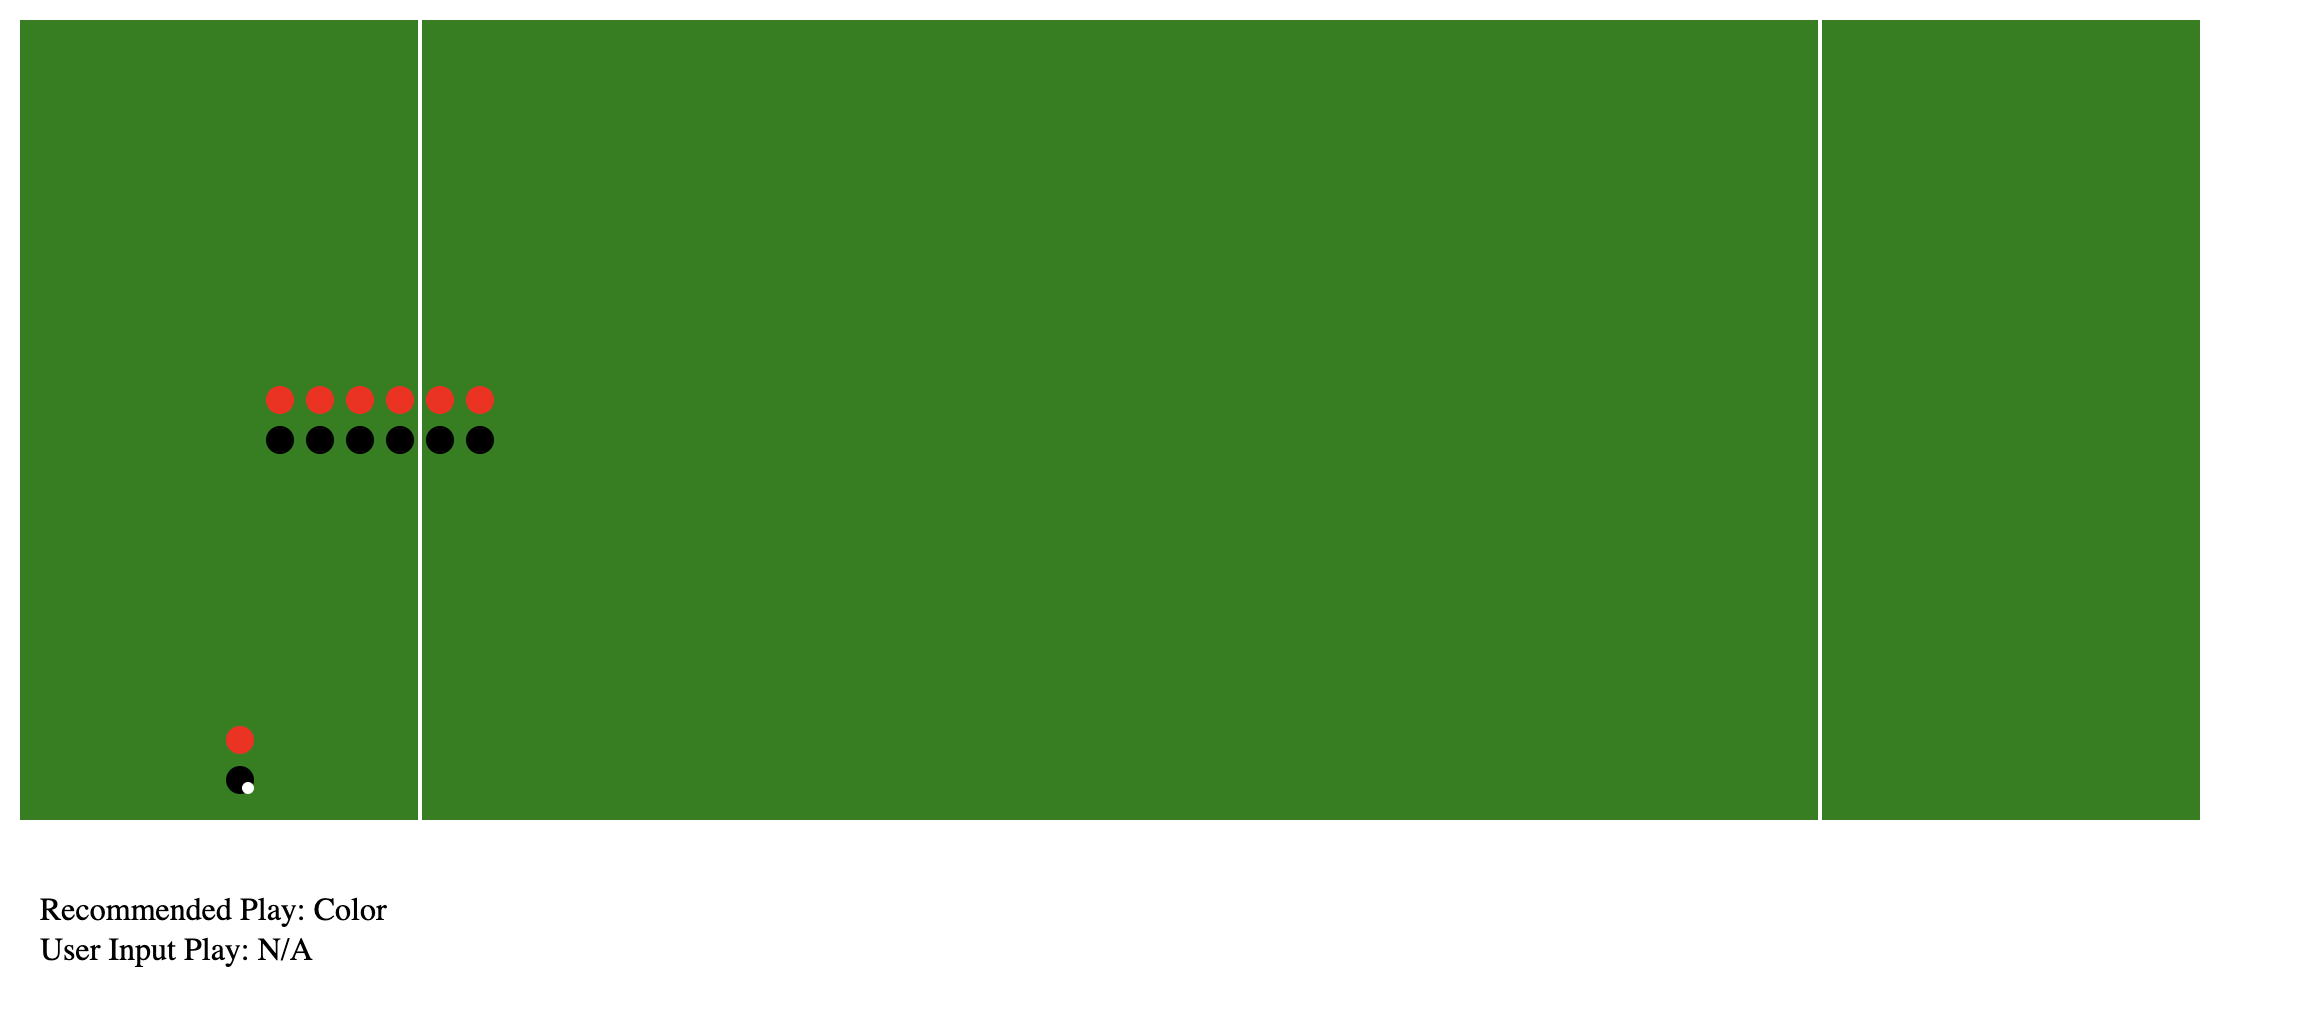
\includegraphics[width=.8\textwidth]{images/basic.png}
    \end{center}
   
    ~\\
    ~\\
    Example 2: Automatic Person Defense (auto.txt)
    ~\\
    \begin{verbatim}
    Offense = {(220,390), true; (220,220), false; (300,220), false; (320,220), false; 
                (340,220), false; (360,220), false; (380,220), false; }
    Defense = Automatic
    Force = Away
    \end{verbatim}
    ~\\
    Running "dotnet run auto.txt \textgreater \  auto.svg" produces an svg file with the image below as output
    \begin{center}
        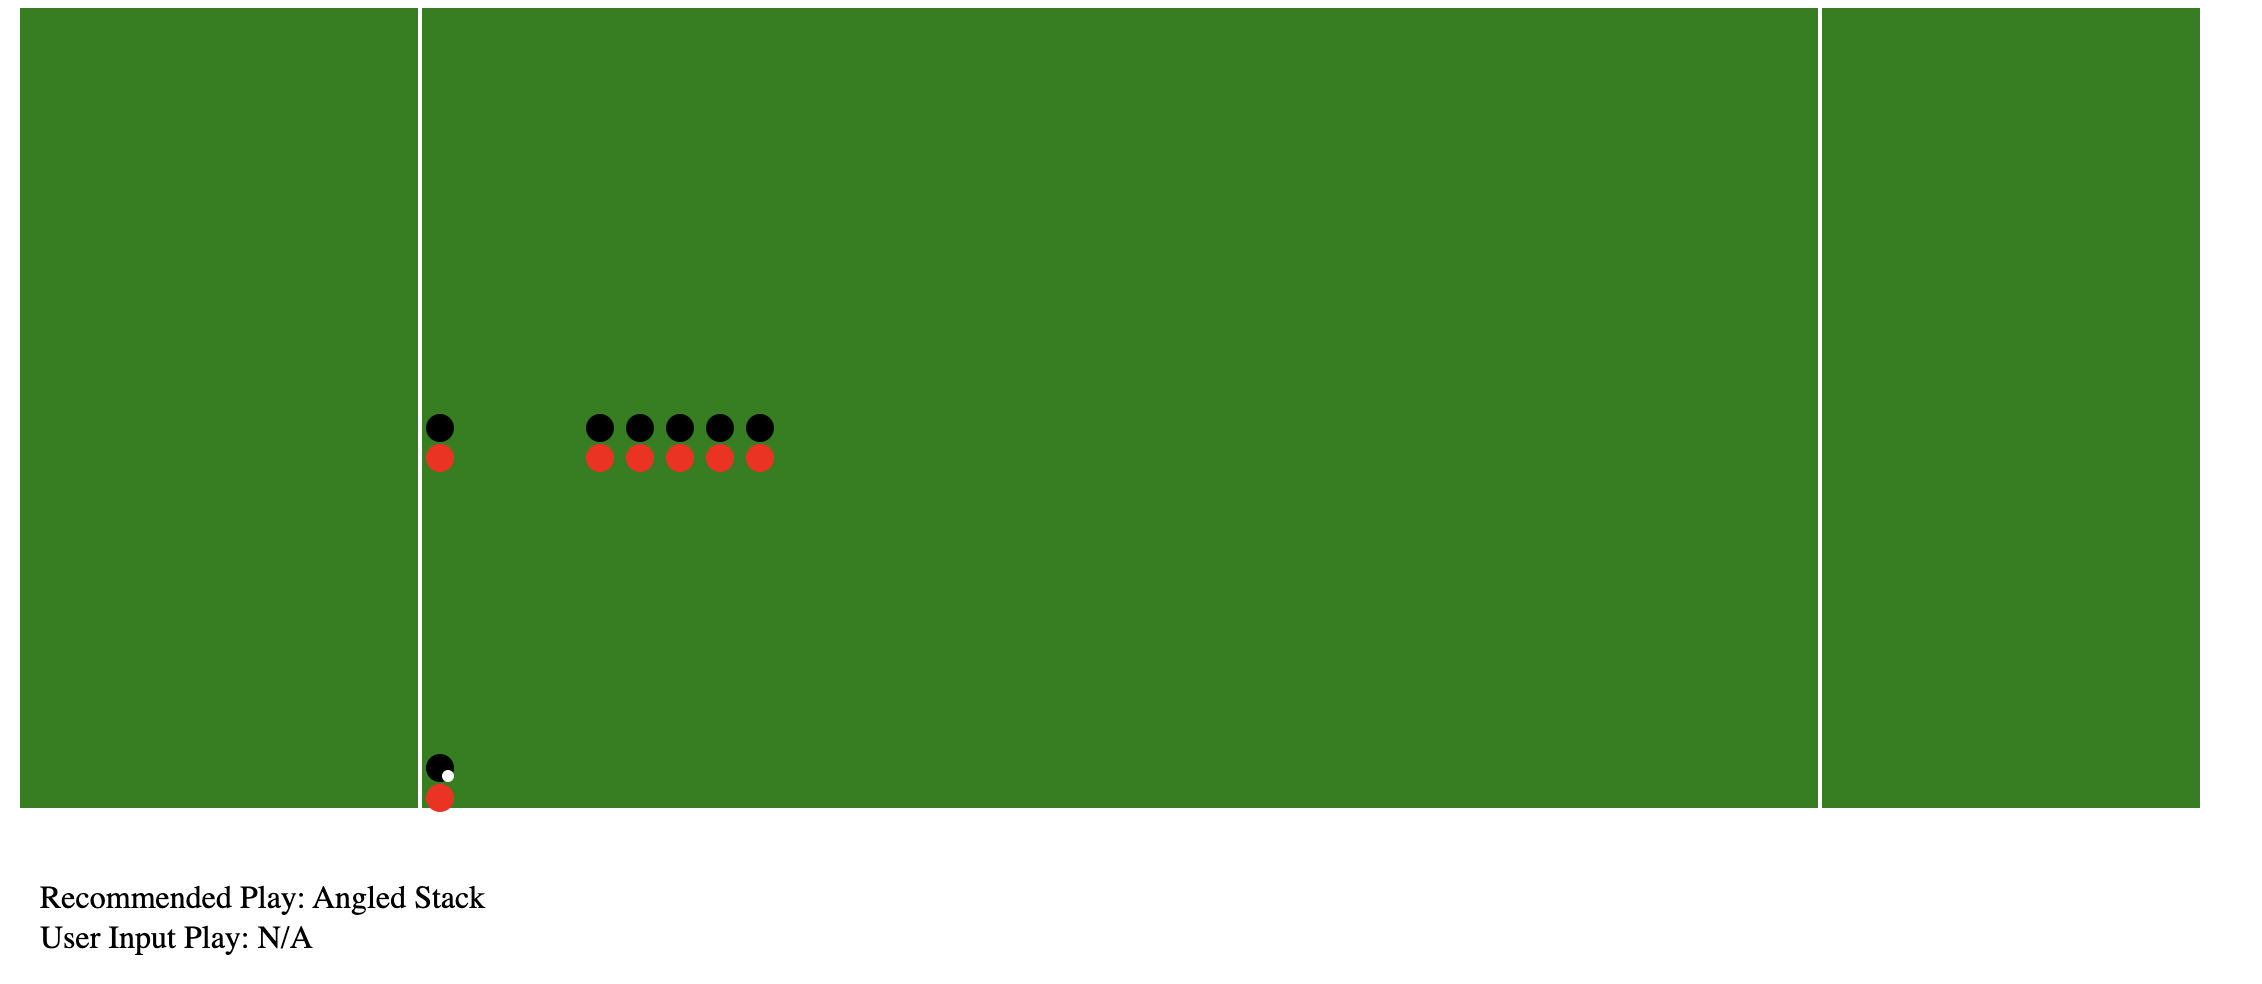
\includegraphics[width=.8\textwidth]{images/auto.png}
    \end{center}

    ~\\
    ~\\
    Example 3: Adding plays (addplay.txt)
    ~\\
    \begin{verbatim}
    Offense = {(220,390), true; (220,270), false; (220,140), false; (400,350), false; 
                (400,275), false; (400,175), false; (400,100), false; }
    Defense = Automatic
    Force = Home
    Play = if disc in range 100 to 300 and force is Force = Home
    \end{verbatim}
    ~\\
    Running "dotnet run addplay.txt \textgreater \  addplay.svg" produces an svg file with the image below as output
    \begin{center}
        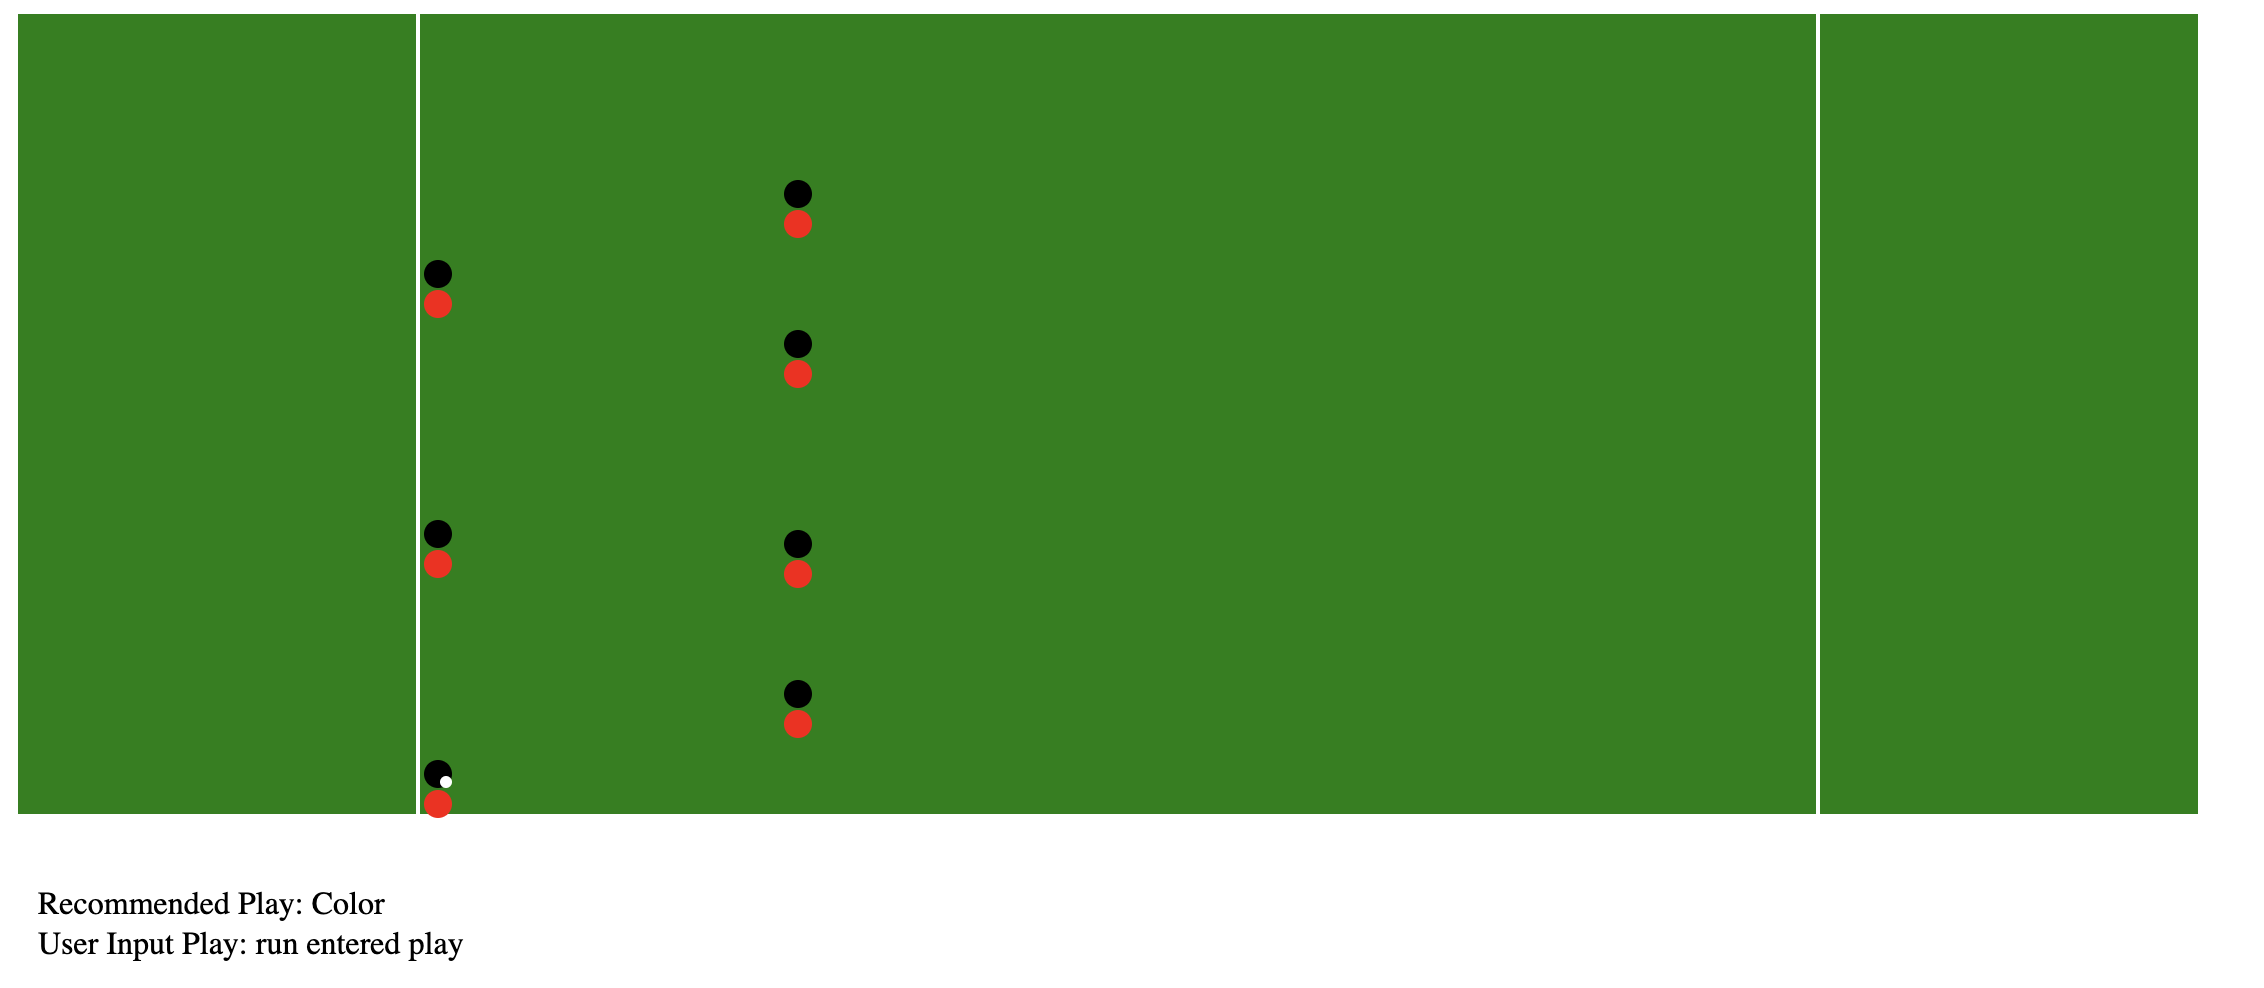
\includegraphics[width=.8\textwidth]{images/addedplay.png}
    \end{center}

\subsection*{Language Concepts}

Programs in frisBRO contain a field, a force, a defense type, and optionally, a list of plays. A field is made up of teams, which are lists of players. Players are made up of coordinates, and for offense, a string of true or false that tracks whether or not the player has the disc. The force is a string that can be one of three options (Home, Away, or Flat) and aids in the calling of plays. The defense is a string that can be Manual or Automatic, depending on how the user intends to populate the defense. The plays are input by the user as a string containing a range, a force, and a name.
~\\
~\\
The primitives in our language are integers, coordinates, and strings, which are combined into players, teams, and the field. In order to understand our program, users should have a good grasp of the game of ultimate - they need to be able to identify the force and estimate where on the field players are. Additionally, in order to input plays, the user should understand when a certain play should be run (e.g., run endzone if within 10 yards of the endzone, run color if on the sideline and force is home, etc).
~\\
Field Visualization: 
\begin{center}
    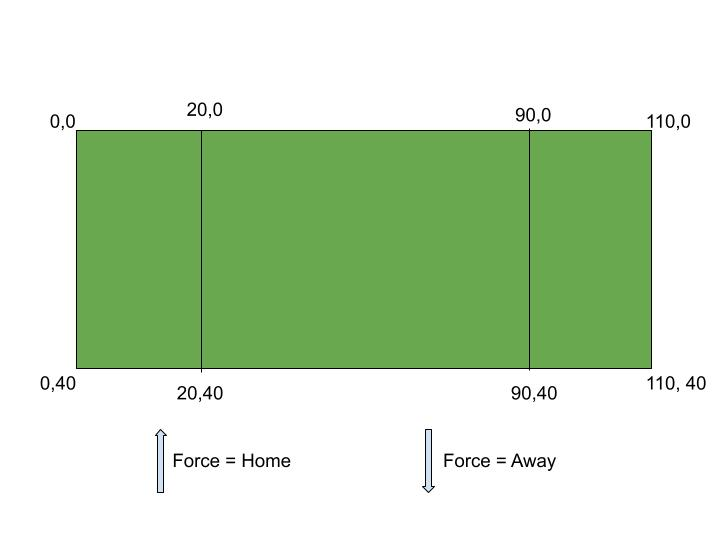
\includegraphics[width=.5\textwidth]{images/FieldVisualization.jpg}
\end{center}

\subsection*{Formal Syntax}


% Current syntax:
% ~\\
%     $<$expr$>$		::=$<$offense$>$$<$defense$>$
%     ~\\
%     $<$offense$>$	::= $<$oplayer$>$$<$offense$>$ $|$ $<$oplayer$>$
%     ~\\
%     $<$defense$>$	::= $<$dplayer$>$$<$defense$>$ $|$ $<$dplayer$>$
%     ~\\
    
%     $<$oplayer$>$ 	::= $<$coordinate$>$$<$disc$>$
%     ~\\
%     $<$dplayer$>$	::= $<$coordinate$>$
%     ~\\
%     $<$disc$>$  	::= true $|$ false
%     ~\\
%     $<$coordinate$>$::= ($<$digit$>$,$<$digit$>$)
%     ~\\
%     $<$digit$>$		    ::= $<$digit$>$n $|$ n  where n is any positive integer
% ~\\
% ~\\

~\\
    $<$expr$>$		::= $<$field$>$$<$plays$>$ $|$ $<$field$>$
    ~\\
    $<$field$>$		::=$<$teams$>$$<$flag$>$$<$force$>$
    ~\\
    $<$teams$>$     ::= $<$offensive$>$$<$defensive$>$
    ~\\
    $<$offensive$>$	::= $<$oplayer$>$$<$offensive$>$ $|$ $<$oplayer$>$
    ~\\
    $<$defensive$>$	::= $<$dplayer$>$$<$defensive$>$ $|$ $<$dplayer$>$  
    ~\\
    $<$hasdisc$>$  	::= true $|$ false
    ~\\
    $<$oplayer$>$ 	::= $<$coordinate$>$$<$hasdisc$>$
    ~\\
    $<$dplayer$>$	::= $<$coordinate$>$
    ~\\
    $<$force$>$ 	::= home $|$ away $|$ flat
    ~\\
    $<$flag$>$      ::= automatic $|$ manual
    ~\\
    $<$plays$>$ 	::= $<$play$>$ $|$ $<$play$>$$<$plays$>$ $|$ Library
    ~\\
    $<$play$>$ 		::= if disc in range $<$digit$>$ to $<$digit$>$ and force is Force = $<$force$>$ with name as $<$playname$>$
    ~\\
    $<$playname$>$  ::= string
    ~\\
    $<$coordinate$>$::= ($<$digit$>$,$<$digit$>$)
    ~\\
    $<$digit$>$		    ::= $<$digit$>$n $|$ n  where n is any positive integer



\subsection*{Semantics}

\begin{center}
    \begin{tabular}{ | m{5cm} | m{5cm}|  m{5cm} |} 
      \hline
      Syntax & Abstract Syntax & Meaning \\ 
      \hline
      $<$n$>$ & Digit of int & n is a primative integer stored using F\# integers \\
      \hline
      ($<$n$>$,$<$n$>$) & Coordinate of {x: int; y: int} & x and y are integers. A coordinate is a primitive that represents where on the field a player is. \\ 
      \hline
      $<$coordinate$>$, $<$hasDisc$>$ & Offense of Coordinate * HasDisc & An offensive player is made up of a coordinate and a boolean value of whether or not they have the disc. The player is drawn on the field in the appropriate location with/without the disc based on this information. \\ 
      \hline
      $<$coordinate$>$ & Defense of Coordinate & A defensive player is made up of a coordinate. The player is drawn on the field in the appropriate location. \\ 
      \hline
      $<$offense$>$ $|$ $<$defense$>$ & Player of Offense or Defense & A player is either on Offense or Defense. Players are used to create Teams which are a list of players\\
      \hline
      ($<$player$>$, $<$offensive$>$) $|$ $<$player$>$ & Offensive of Player list & Offensive (which symbolizes an offensive team) is a list of offensive players. This is a combining form of offense players. \\
      \hline
      ($<$player$>$, $<$defensive$>$) $|$ $<$player$>$ & Defensive of Player list & Defensive (which symbolizes an defensive team) is a list of defensive players. This is a combining form of defense players. \\
      \hline
      True $|$ False & HasDisc of True or False & A boolean primative which determines if an offense player has a disc. \\
      \hline
      Automatic $|$ Manual & Flag of Automatic or Manual & A primative which determines if user put in their own defense or automatically populated it. \\
      \hline
      Home $|$ Away $|$ Flat & Force of Home or Away or Flat & A primative which tells the program what the force is on the field. \\
      \hline
      if disc in range $<$n$>$ to $<$n$>$ and force = $<$force$>$ with name as $<$string$>$ & Play of (int * int) * Force * Name & A combining form which combines the users inputted play based on a range and a force into a Play type. \\
      \hline
      Offense = $<$offensive$>$ Defense = $<$defensive$>$ $|$ $<$flag$>$ Force = $<$force$>$ Play = $<$plays$>$ & Field of Team list * Flag * Force * Play list & The final combining form which collects all user input into a usable tuple \\
      \hline
    \end{tabular}
\end{center}

\subsection*{Remaining Work}

While we believe that this language would help ultimate frisbee players in this current
iteration, some improvements could be made to increase functionality. We would like to add arrows that represent where each player should move in the recommended play. This would allow the user to more clearly visualize the suggested play. Additionally, we would like to give the user the ability to add more detailed conditions for the plays they enter. For example, 
the user could specify where the disc is on the field vertically, not just horizontally. Currently, when the user asks for defense to be placed automatically, they are placed in a person defense. We'd like to add automatic zone defense as an option in the future. Finally, we would like to build more plays into the language as a baseline, so the recommendations are more helpful and specific.

% DO NOT DELETE ANYTHING BELOW THIS LINE
\end{document}
